% Results section: Uncertainty Quantification for pediatric bone age regression.
% Self-contained, compilable document. Can also be \input{} into a larger report
% by reusing the body between \begin{document} and \end{document}.
% Requires report/figures/uq_results_comparison.pdf (generated by
% report/figures/make_results_figure.py).
\documentclass[11pt]{article}

\usepackage[utf8]{inputenc}
\usepackage[T1]{fontenc}
\usepackage{amsmath}
\usepackage{amssymb}
\usepackage{graphicx}
\usepackage{booktabs}
\usepackage{siunitx}
\usepackage{geometry}
\usepackage[hidelinks]{hyperref}

\geometry{margin=1in}
\graphicspath{{figures/}}

\newcommand{\code}[1]{\texttt{#1}}

\title{Uncertainty Quantification for Pediatric Bone Age Regression:\\ Results}
\author{}
\date{}

\begin{document}

\maketitle

\section{Results}

\subsection{How the Metrics Were Acquired}

All numbers reported below are computed on the external RSNA held-out test split
($N = 1425$ radiographs), which is never seen during training or calibration.
Each method follows the same three-stage protocol described in the Methodology:
a model is trained and its best checkpoint restored; a single post-hoc
temperature scalar $s$ is fit on the disjoint calibration split; and the test
split is then evaluated with that $s$ applied. For the sampling-based
configurations (MC Dropout), the predictive mean and standard deviation are
obtained from $T = 30$ stochastic forward passes; the heteroscedastic model
produces its mean and standard deviation in a single deterministic pass.

From the per-sample mean $\mu_i$ and (calibrated) standard deviation
$\sigma_i^{\text{eff}} = s\,\sigma_i$, Gaussian prediction intervals
$\mu_i \pm z_c\,\sigma_i^{\text{eff}}$ are built at the $90\%$ ($z = 1.645$) and
$95\%$ ($z = 1.960$) levels. Every prediction is de-normalized back to months
before scoring. We report four families of metrics, all in month space:
point accuracy via the mean absolute error (MAE) and root-mean-square error
(RMSE) of $\mu_i$; calibration via the Prediction Interval Coverage Probability
(PICP), the empirical fraction of true ages falling inside their intervals; and
sharpness via the Mean Prediction Interval Width (MPIW). A well-calibrated
method has PICP close to its nominal level (90\% or 95\%); among methods with
comparable coverage, a smaller MPIW indicates tighter, more informative
intervals. The per-method metrics rows are emitted by the shared evaluation
code and aggregated into a single ranked comparison table.

\subsection{Quantitative Comparison}

Table~\ref{tab:results} reports the test-split results for the evaluated
configurations, and Figure~\ref{fig:results} visualizes the same data, split
into calibration (coverage) and sharpness (width) views.

\begin{table}[htbp]
  \centering
  \caption{Test-split uncertainty quantification results ($N = 1425$). PICP and
  MPIW are reported at the $90\%$ and $95\%$ nominal levels. Point-accuracy
  metrics (MAE, RMSE) describe the mean prediction; coverage closest to nominal
  with the smallest width is preferable.}
  \label{tab:results}
  \begin{tabular}{lcccc}
    \toprule
    \textbf{UQ Method} & \textbf{MAE} & \textbf{RMSE} & \textbf{PICP (90 / 95)} & \textbf{MPIW (90 / 95)} \\
                       & (months)     & (months)      & (\%)                     & (months) \\
    \midrule
    MC Dropout (Uncalibrated)    & 7.50 & 10.01 & 78.74 / 83.51 & 27.73 / 33.04 \\
    MC Dropout (Calibrated)      & 7.50 & 10.01 & 92.98 / 95.79 & 54.22 / 64.61 \\
    UQ-Aware Trained MC Dropout  & 8.61 & 11.20 & 89.12 / 93.47 & 40.69 / 48.48 \\
    Heteroscedastic              & 8.65 & 11.17 & 90.11 / 94.11 & 35.35 / 42.12 \\
    \bottomrule
  \end{tabular}
\end{table}

\begin{figure}[htbp]
  \centering
  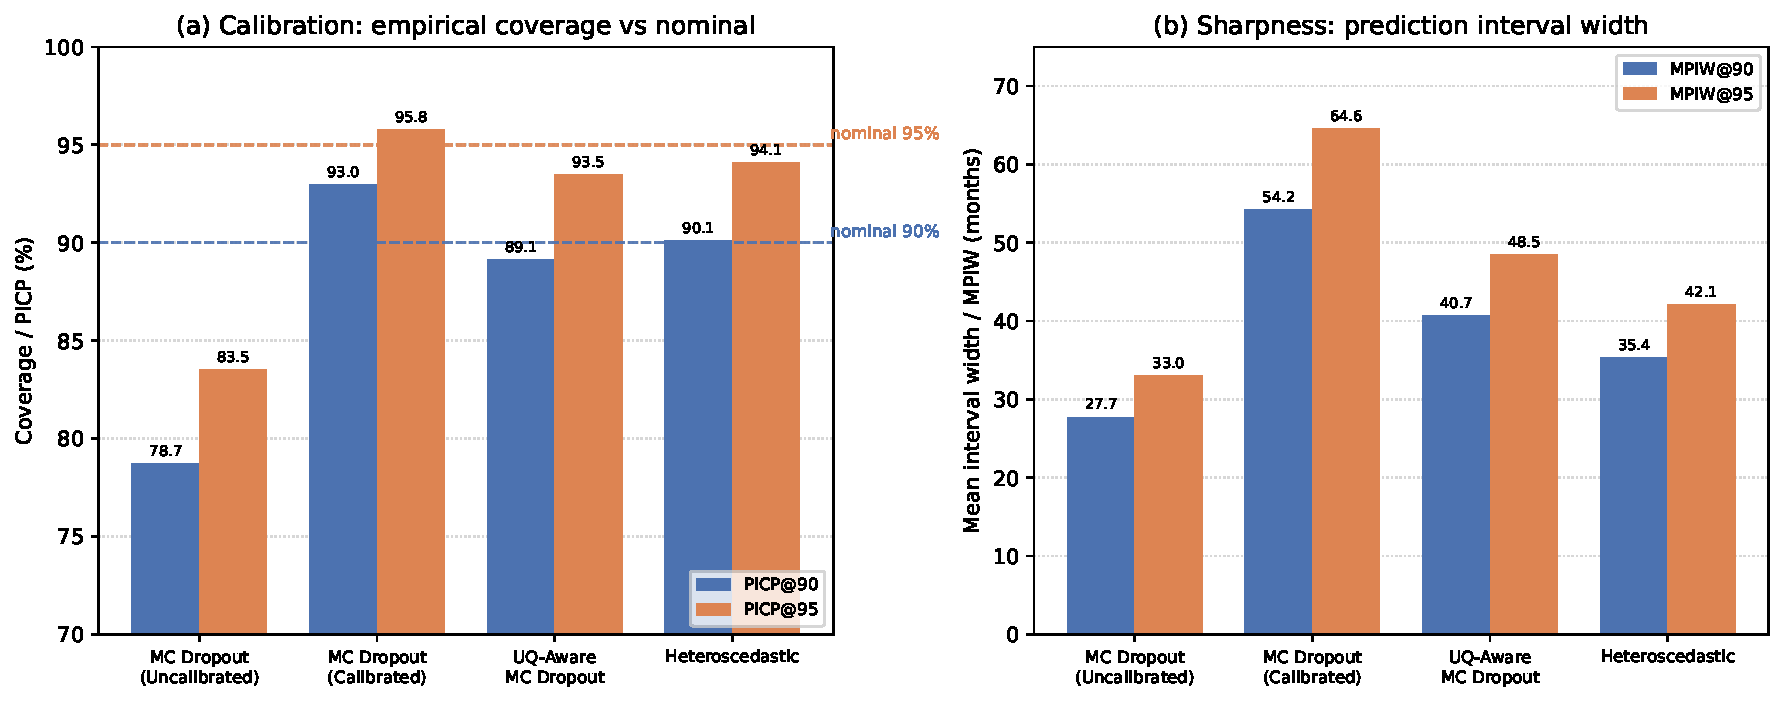
\includegraphics[width=\textwidth]{uq_results_comparison.pdf}
  \caption{Test-split comparison of the UQ configurations. (a) Empirical
  coverage (PICP) against the nominal $90\%$ and $95\%$ levels (dashed lines);
  bars near the lines indicate good calibration. (b) Mean prediction interval
  width (MPIW); shorter bars indicate sharper intervals. The calibrated MC
  Dropout configuration reaches nominal coverage but with the widest intervals,
  whereas the heteroscedastic model attains comparable coverage with markedly
  narrower intervals.}
  \label{fig:results}
\end{figure}

\subsection{Analysis}

\paragraph{Calibration is essential.} Out of the box, MC Dropout is badly
under-confident: its raw $90\%$ intervals cover only $78.7\%$ of test cases
(and $83.5\%$ at the $95\%$ level), well below nominal. This is a direct
consequence of the architecture exposing a single head dropout layer, which
produces too small a predictive spread. Post-hoc temperature scaling corrects
this almost exactly---calibrated coverage rises to $93.0\%$ / $95.8\%$, within
roughly one point of nominal---confirming that a single scalar fit on the
held-out calibration split is sufficient to repair coverage. Crucially, point
accuracy is unchanged (MAE $= 7.50$ months in both rows), since temperature
scaling only rescales the interval width and not the mean prediction.

\paragraph{Coverage has a price in width.} Calibration achieves correct coverage
only by widening the MC Dropout intervals substantially, from $27.7$ to $54.2$
months at the $90\%$ level. Coverage and sharpness are therefore competing
objectives: the uncalibrated intervals are narrow but untrustworthy, while the
calibrated ones are trustworthy but the least informative of the methods.

\paragraph{Training for uncertainty trades a little accuracy for much tighter
intervals.} The UQ-aware trained MC Dropout, whose checkpoint is selected for
calibrated interval quality rather than plain validation error, reaches near
nominal coverage ($89.1\%$ / $93.5\%$) with $90\%$ intervals of $40.7$ months,
about a quarter narrower than the post-hoc-calibrated baseline. This comes at a
modest cost in point accuracy (MAE $8.61$ vs.\ $7.50$ months), illustrating the
expected trade-off between optimizing for the mean and optimizing for the full
predictive distribution.

\paragraph{The heteroscedastic model offers the best calibration-sharpness
balance.} The heteroscedastic regressor attains the coverage closest to nominal
($90.1\%$ / $94.1\%$, a $90\%$ calibration error of only $\sim$0.1 points) while
producing the narrowest intervals among the well-calibrated methods ($35.4$ /
$42.1$ months). Because it predicts an input-dependent variance in a single
forward pass, it is also the cheapest method at inference time. Its point
accuracy ($8.65$ months MAE) is essentially tied with the UQ-aware MC Dropout
model and slightly behind the deterministic mean of the base network. On the
guiding criterion---coverage close to nominal, then smallest width---the
heteroscedastic model is the strongest of the evaluated configurations.

\paragraph{Summary.} The base network already provides accurate point estimates
($\approx$7.5 months MAE), but its raw dropout uncertainty is not trustworthy
without calibration. Once calibrated, all configurations reach approximately
nominal coverage; they then differ chiefly in sharpness, where uncertainty-aware
training and, especially, the heteroscedastic formulation deliver substantially
more informative intervals than post-hoc calibration of the base model alone.

\paragraph{Note on the Bayesian Neural Network.} The BNN configuration is
omitted from Table~\ref{tab:results}: only a smoke-test checkpoint (2 epochs on
$1\%$ of the data) was available, which had not converged (test MAE $\approx 82$
months, $R^2 < 0$) and therefore does not provide a meaningful comparison. A
fully trained BNN run is left to future work.

\end{document}
